\chapter{Datasets}
To test our extraction-classification pipeline, we use three progressively more complex datasets. We start by classifying simple 2D shapes, then move on to simple 3D shapes, and last, we attempt to classify a dataset of real photographs of cats and dogs.

Each dataset is split into a training and a testing subset. This ensures that we can test, how the classifier performs on unseen data.

\section{2D Shapes Dataset}\label{sec:2d-dataset}
For the simplest dataset, we use a four shapes dataset \cite{kaggleFourShapes}. The dataset contains $16$,$000$ images of four shapes: square, star, circle, and triangle. The dataset was created from poster board cutouts of each shape painted green. While rotating, each shape was recorded using a Garmin Virb 1080p action camera for two minutes. Shapes were then cropped out from the frames of the video and resized to $200\times200$ pixels. The green color of the cutouts in frames was then changed to a pure black color, while the rest of the image was changed to a pure white color. An example of the data can be seen in \figref{fig:four_shapes}.
\begin{figure}[ht!]
    \centering
    \begin{subfigure}[t]{0.25\textwidth}
        
\includegraphics[width=\textwidth]{Figures/datasets/circle.png}
        \caption{Circle}
    \end{subfigure}
    \begin{subfigure}[t]{0.25\textwidth}
        
\includegraphics[width=\textwidth]{Figures/datasets/star.png}
        \caption{Star}
    \end{subfigure}
    \caption[Photographs of a circle and a star from the Four Shapes dataset]{Photographs of a circle and a star from the Four Shapes dataset \cite{kaggleFourShapes}.}
    \label{fig:four_shapes}
\end{figure}

Since we are interested in binary classification, we use only the pair of a circle (positive class) and a star (negative class). We assign $\sfrac{2}{3}$ of random images from each class to a training subset, and $\sfrac{1}{3}$ to a testing subset.

\section{3D Shapes Dataset}\label{sec:3d-dataset}
The 3D Shapes dataset contains $20$ images of a box (positive class) and $20$ images of a sphere (negative class) viewed from different angles. The shapes are colored red, while the background is colored white. The objects are illuminated by a single light source, providing a nice and sharp shadow and shading of each shape. The dataset was generated by Ing. Lukáš Pospíšil, Ph.D. using POV-Ray software \cite{povray}. Each of the images is $300\times200$ pixels. An example of each shape can be seen in \figref{fig:3d_shapes}.
\begin{figure}[ht]
    \centering
    \begin{subfigure}[t]{0.3\textwidth}
        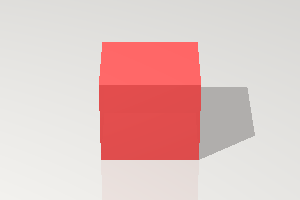
\includegraphics[width=\textwidth]{Figures/datasets/box.png}
        \caption{Box}
    \end{subfigure}
    \begin{subfigure}[t]{0.3\textwidth}
        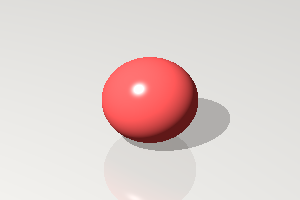
\includegraphics[width=\textwidth]{Figures/datasets/sphere.png}
        \caption{Sphere}
    \end{subfigure}
    \caption[3D shapes, generated by Ing. Lukáš Pospíšil, Ph.D. in POV-Ray]{3D shapes, generated by Ing. Lukáš Pospíšil, Ph.D. in POV-Ray \cite{povray}.}
    \label{fig:3d_shapes}
\end{figure}

We assign $\sfrac{2}{3}$ of random images from each class to a training subset, and $\sfrac{1}{3}$ to a testing subset.

\section{Cats and Dogs Dataset}\label{sec:cat_dog_dataset}
The Cats and Dogs dataset is created from the Oxford-IIIT Pet Dataset \cite{parkhi12a}. Since the original dataset contains a few damaged images, we use a fixed version of the dataset from \cite{ml4py_dataset}.

The dataset contains over $7$,$000$ images of different cat and dog breeds, example of a cat and a dog image can be seen in \figref{fig:iiit_pet}.
\begin{figure}[!ht]
    \centering
    \begin{subfigure}[t]{0.45\textwidth}
        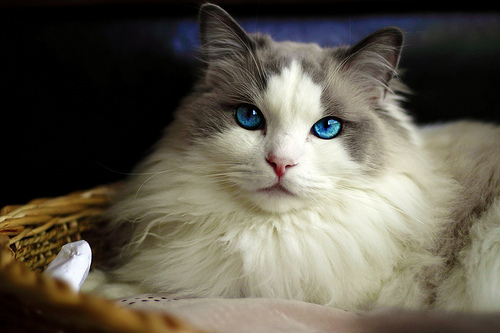
\includegraphics[width=\textwidth]{Figures/datasets/cat.jpg}
        \label{fig:original:example_cat}
    \end{subfigure}\hfill
    \begin{subfigure}[t]{0.45\textwidth}
        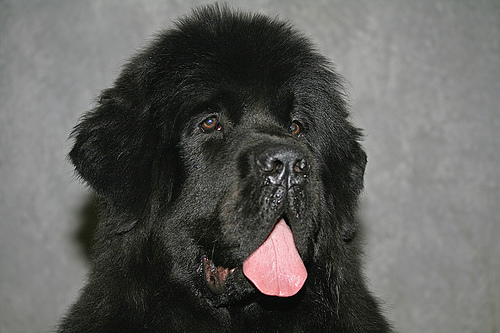
\includegraphics[width=\textwidth]{Figures/datasets/dog.jpg}
        \label{fig:original:example_dog}
    \end{subfigure}
    \caption[Example of images depicting a cat (left) and a dog (right) in the Oxford-IIIT Pet Dataset]{Example of images depicting a cat (left) and a dog (right) in the Oxford-IIIT Pet Dataset \cite{parkhi12a}.}
    \label{fig:iiit_pet}
\end{figure}
The classes in the dataset are unbalanced, there are approximately twice as many images of dogs than images of cats.

The dataset provides us with a trimap for each image. The trimap consists of the information, which of the pixels are of the animal and which are of the background. We use these to cut out the animal from the background (set all the background pixel values to black). An example is demonstrated in \figref{fig:iiit_pet_cutout}.
\begin{figure}[!ht]
    \centering
    \begin{subfigure}{0.55\textwidth}
        \begin{subfigure}[t]{0.40\textwidth}
            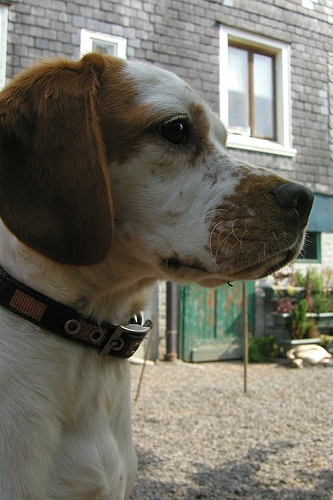
\includegraphics[width=\textwidth]{Figures/datasets/beagele.jpg}
            \label{fig:original:example}
        \end{subfigure}\hfill
        \begin{subfigure}[t]{0.40\textwidth}
            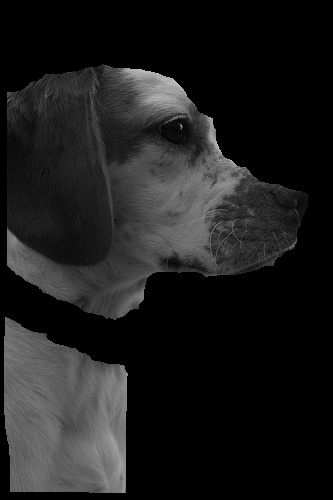
\includegraphics[width=\textwidth]{Figures/datasets/beagle_nobkg.jpg}
            \label{fig:pet:example}
        \end{subfigure}
    \end{subfigure}
    \caption[Original of a photograph of a beagle (left) and a cutout (right).]{Original of a photograph of a beagle (left) and a cutout (right) \cite{parkhi12a}.}
    \label{fig:iiit_pet_cutout}
\end{figure}

We assign the positive class to images of cats, and the negative class to images of dogs. In the original dataset,` we are provided with a training and testing subset. However, the ratio of training and testing samples in these classes is approximately $1:1$. To get a better representation of the data, we split the dataset ourselves, where we assign $90\%$ of the data to a training subset and $10\%$ of the data to a testing subset. The data is selected at random, making sure that for each breed of a cat or a dog, the ratio of amounts of training samples to testing samples is kept the same.
